
%----------------------------------------------------------------------------------------
%	PACKAGES AND OTHER DOCUMENT CONFIGURATIONS
%----------------------------------------------------------------------------------------

\documentclass[final]{beamer}

\usepackage[scale=1.24]{beamerposter} % Use the beamerposter package for laying out the poster

\usetheme{confposter} % Use the confposter theme supplied with this template

\setbeamercolor{block title}{fg=ngreen,bg=white} % Colors of the block titles
\setbeamercolor{block body}{fg=black,bg=white} % Colors of the body of blocks
\setbeamercolor{block alerted title}{fg=white,bg=dblue!70} % Colors of the highlighted block titles
\setbeamercolor{block alerted body}{fg=black,bg=dblue!10} % Colors of the body of highlighted blocks
% Many more colors are available for use in beamerthemeconfposter.sty

%-----------------------------------------------------------
% Define the column widths and overall poster size
% To set effective sepwid, onecolwid and twocolwid values, first choose how many columns you want and how much separation you want between columns
% In this template, the separation width chosen is 0.024 of the paper width and a 4-column layout
% onecolwid should therefore be (1-(# of columns+1)*sepwid)/# of columns e.g. (1-(4+1)*0.024)/4 = 0.22
% Set twocolwid to be (2*onecolwid)+sepwid = 0.464
% Set threecolwid to be (3*onecolwid)+2*sepwid = 0.708

\newlength{\sepwid}
\newlength{\onecolwid}
\newlength{\twocolwid}
\newlength{\threecolwid}
\setlength{\paperwidth}{48in} % A0 width: 46.8in
\setlength{\paperheight}{36in} % A0 height: 33.1in
% \setlength{\paperwidth}{36in} % A1 width: 33.1in
% \setlength{\paperheight}{25in} % A1 height: 23.4in
\setlength{\sepwid}{0.024\paperwidth} % Separation width (white space) between columns
% \setlength{\sepwid}{0.0342\paperwidth} 
\setlength{\onecolwid}{0.22\paperwidth} % Width of one column in two column mode
\setlength{\onecolwid}{0.22\paperwidth} % Width of one column
\setlength{\twocolwid}{0.464\paperwidth} % Width of two columns
\setlength{\threecolwid}{0.708\paperwidth} % Width of three columns
\setlength{\topmargin}{-0.5in} % Reduce the top margin size
%-----------------------------------------------------------

\usepackage{graphicx}  % Required for including images

\usepackage{booktabs} % Top and bottom rules for tables

\newtheorem*{rawnamedtheorem}{\therawnamedtheorem}
\newcommand{\therawnamedtheorem}{\error}
\newenvironment{namedtheorem}[1]{\renewcommand{\therawnamedtheorem}{#1}
   \begin{rawnamedtheorem}}
  {\end{rawnamedtheorem}}

%----------------------------------------------------------------------------------------
%	TITLE SECTION 
%----------------------------------------------------------------------------------------

\title{Securing Shards with only 10 Validators} % Poster title

\author{Handan Kılınç Alper, Jeff Burdges, Robert Habermeier, Seyed Hosseini, Alistair Stewart} % Author(s)

\institute{Web 3.0 Foundation} % Institution(s)

%----------------------------------------------------------------------------------------

\begin{document}

\addtobeamertemplate{block end}{}{\vspace*{2ex}} % White space under blocks
\addtobeamertemplate{block alerted end}{}{\vspace*{2ex}} % White space under highlighted (alert) blocks

\setlength{\belowcaptionskip}{2ex} % White space under figures
\setlength\belowdisplayshortskip{2ex} % White space under equations

\begin{frame}[t] % The whole poster is enclosed in one beamer frame

\begin{columns}[t] % The whole poster consists of three major columns, the second of which is split into two columns twice - the [t] option aligns each column's content to the top

\begin{column}{\sepwid}\end{column} % Empty spacer column

\begin{column}{\onecolwid} % The first column

%----------------------------------------------------------------------------------------
%	OBJECTIVES
%----------------------------------------------------------------------------------------

\begin{alertblock}{Goal}

A sharded blockchain in which the shards trust one another but shards cost relatively little.

\end{alertblock}

%----------------------------------------------------------------------------------------
%	INTRODUCTION
%----------------------------------------------------------------------------------------

\begin{block}{Literature}

Almost all sharding designs attempt to overwhelm the problem with the shear number of validators: \\
\begin{itemize}
\item Cosmos ignores overlap entirely
\item ETH 2.0 wants 300-1000 validators per shard..  with every 32 ETH being a validator
\item OmniLedger similar
\end{itemize}

\medskip

Machines are cheap, but independence is not: \\ 
\hspace*{5pt}  operators, data centers, etc.

\bigskip

\textbf{Scalable?}

How many validators can I run on one machine?  How many P2P networks?  How much bandwidth?

\bigskip

\textbf{Secure?}

At best, we require much more than 1/3rd honest, \\
\hspace*{5pt}  but even 1/3rd honest sounds dubious.

\bigskip
\bigskip
\bigskip

\begin{figure}

\includegraphics[width=0.8\linewidth]{eliminate-small.jpg}
% \caption{Eliminate the state}
\end{figure}

\bigskip

Real sharding requires validation by light clients, \\
\hspace*{5pt} at the extreme called ``fishermen''.

\bigskip

\textbf{Idea}:  Attach Merklee proofs for the state root, \\
\hspace*{5pt}  creating proof-of-validity (PoV) blocks.

\bigskip

PoV block allow validation by light clients \\ who lack any chain state.

\bigskip
\bigskip

\textbf{Idea}:  Random checks are independent, \\
\hspace*{5pt} which inverts the adversary's statistical advantage.

\bigskip
\bigskip

\textbf{How to manage these ``fraud proofs''?}

\end{block}

%----------------------------------------------------------------------------------------

\end{column} % End of the first column

\begin{column}{\sepwid}\end{column} % Empty spacer column

\begin{column}{\twocolwid} % Begin a column which is two columns wide (column 2)

\begin{columns}[t,totalwidth=\twocolwid] % Split up the two columns wide column

\begin{column}{\onecolwid}\vspace{-.6in} % The first column within column 2 (column 2.1)

%----------------------------------------------------------------------------------------
%	MATERIALS
%----------------------------------------------------------------------------------------

\begin{block}{Availability}

% Any random checks by the (light client) fishermen still require the block being checked.
% 
% \bigskip

In \cite{FraudProofs}, a two dimensional Reed-Solomon trick ensures 
fishermen reconstruct bock fragments, so

\begin{itemize}
\item violation is distributed across fishermen, \\ which scales nicely,
\item but short fraud proofs sound irrelevant.
\end{itemize}

\bigskip On the other hand..

\begin{itemize}
\item Accessing state remains tricky.. \\
Too many PoV Merklee proofs reduce scaling.
\item Validation is often non-local.. \\
signature aggregation, big transaction, ..
\end{itemize}

\bigskip
\bigskip

Needs $> 3/4$ honest if block validation is non-local!

\end{block}

% \begin{namedtheorem}{Alistair's trick}
% Integrate erasure coding with the finality gadget.
% \end{namedtheorem}

%----------------------------------------------------------------------------------------

\end{column} % End of column 2.1

\begin{column}{\onecolwid}\vspace{-.6in} % The second column within column 2 (column 2.2)

%----------------------------------------------------------------------------------------
%	METHODS
%----------------------------------------------------------------------------------------

\begin{block}{Alistair's trick}

We convince the $n$ validators % of a relay aka hub chain
that they could reconstruct the shards' blocks, but
without providing each shard to all $n$.

\bigskip

Reed-Solomon encode blocks 
\begin{itemize}
\item reconstruct from any $\lfloor n/3 \rfloor$,
\item provide validators with distinct shares, 
\end{itemize}

We've a ``relay'' aka hub chain with a finality gadget for which
\begin{itemize}
\item an honest validators $V$ only vote for block $B$ if all $V$ has its share for all shards referenced by $B$.
\end{itemize}

Tolerates $1/3$ Byzantine before finality \\
\hspace*{5pt} and a separate $1/3$ Byzantine after finality

\bigskip
\bigskip

\textbf{Caveot}: Shares cannot be gossiped!

\end{block}

%----------------------------------------------------------------------------------------

\end{column} % End of column 2.2

\end{columns} % End of the split of column 2 - any content after this will now take up 2 columns width

%----------------------------------------------------------------------------------------
%	IMPORTANT RESULT
%----------------------------------------------------------------------------------------

% \setbeamercolor{block alerted title}{fg=white,bg=dblue!70} 
\setbeamercolor{block alerted body}{fg=black,bg=dblue!30} 

\begin{alertblock}{}
\begin{figure}
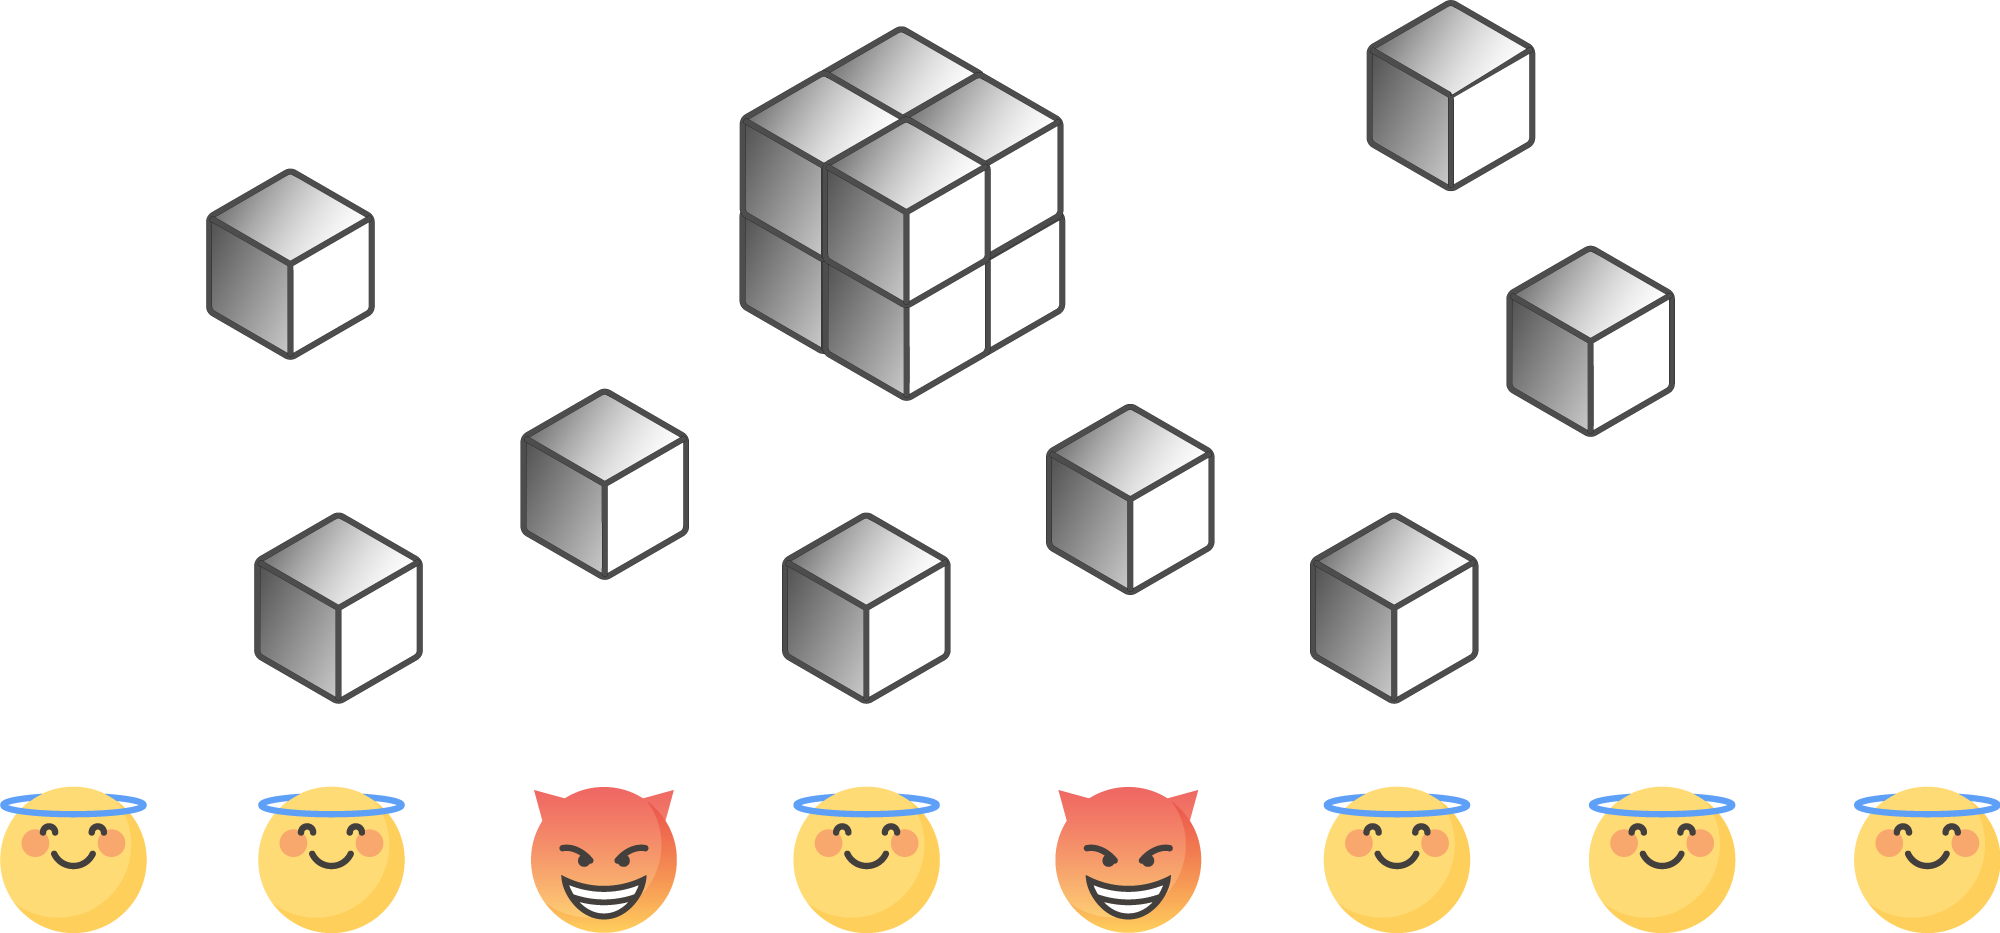
\includegraphics[width=0.8\linewidth]{rob-image1.png}
% \caption{Figure caption}
\end{figure}
\end{alertblock} 

% \setbeamercolor{block alerted title}{fg=white,bg=dblue!70} % Colors of the highlighted block titles
\setbeamercolor{block alerted body}{fg=black,bg=dblue!10} % Colors of the body of highlighted blocks

%----------------------------------------------------------------------------------------

\begin{columns}[t,totalwidth=\twocolwid] % Split up the two columns wide column again

\begin{column}{\onecolwid} % The first column within column 2 (column 2.1)

%----------------------------------------------------------------------------------------
%	MATHEMATICAL SECTION
%----------------------------------------------------------------------------------------

% \begin{block}{Math}
%
% \end{block}

%----------------------------------------------------------------------------------------

\end{column} % End of column 2.1

\begin{column}{\onecolwid} % The second column within column 2 (column 2.2)

%----------------------------------------------------------------------------------------
%	RESULTS
%----------------------------------------------------------------------------------------

% \begin{block}{Results}
%
% \end{block}

%----------------------------------------------------------------------------------------

\end{column} % End of column 2.2

\end{columns} % End of the split of column 2

\end{column} % End of the second column

\begin{column}{\sepwid}\end{column} % Empty spacer column

\begin{column}{\onecolwid} % The third column

%----------------------------------------------------------------------------------------
%	CONCLUSION
%----------------------------------------------------------------------------------------

\begin{block}{Validity}

Availability does nothing without extra validations. \\ \smallskip
We need full blocks for these extra validations, so \\ \smallskip
honest shards should send full blocks when asked, \\ \smallskip
but reconstruction remains a DoS vector.

\bigskip
\bigskip

\textbf{Idea}:  Self-election by VRF so that \\
nodes prove their extra validation rights

\newcommand{\sk}{\ensuremath{\mathsf{sk}}} %secret key
\newcommand{\pv}{\ensuremath{\mathcal{P}V}}
\newcommand{\V}{\ensuremath{\mathcal{V}}}
\newcommand{\vcheck}{\ensuremath{\#V\mathsf{check}}} %number of validity check

\begin{equation}
\mathrm{shardidx} = \mathtt{VRF}_{\sk}(\mathrm{bpvrf}) \mod |\mathrm{shards}|
\end{equation}

\begin{equation}
H(\mathrm{shardidx} \, || \, \mathtt{VRF}_{\sk}(\mathrm{bpvrf})) < \cdots
\end{equation}


\end{block}

%----------------------------------------------------------------------------------------
%	ADDITIONAL INFORMATION
%----------------------------------------------------------------------------------------

% \begin{block}{Additional Information}
%
% \end{block}

%----------------------------------------------------------------------------------------
%	REFERENCES
%----------------------------------------------------------------------------------------

\begin{block}{References}

\nocite{*} % Insert publications even if they are not cited in the poster
\small{\bibliographystyle{unsrt}
\bibliography{background}\vspace{0.75in}}

\end{block}

%----------------------------------------------------------------------------------------
%	ACKNOWLEDGEMENTS
%----------------------------------------------------------------------------------------

% \setbeamercolor{block title}{fg=red,bg=white} % Change the block title color

% \begin{block}{Acknowledgements}

% \small{\rmfamily{Nam mollis tristique neque eu luctus. Suspendisse rutrum congue nisi sed convallis. Aenean id neque dolor. Pellentesque habitant morbi tristique senectus et netus et malesuada fames ac turpis egestas.}} \\

% \end{block}

%----------------------------------------------------------------------------------------
%	CONTACT INFORMATION
%----------------------------------------------------------------------------------------

\setbeamercolor{block alerted title}{fg=black,bg=norange} % Change the alert block title colors
\setbeamercolor{block alerted body}{fg=black,bg=white} % Change the alert block body colors

\begin{alertblock}{Contact Information}

\begin{itemize}
\item Web: \href{https://research.web3.foundation/}{https://research.web3.foundation/}
\item Email: \href{mailto:jeff@web3.foundation}{johnjeff@web3.foundation}
\end{itemize}

\end{alertblock}

\begin{center}
\begin{tabular}{ccc}
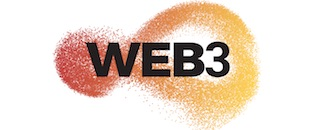
\includegraphics[width=0.4\linewidth]{web3-logo.jpg} & \hfill & 
\includegraphics[width=0.4\linewidth]{polkadot-logo-1.jpg}
\end{tabular}
\end{center}

%----------------------------------------------------------------------------------------

\end{column} % End of the third column

\end{columns} % End of all the columns in the poster

\end{frame} % End of the enclosing frame

\end{document}
\endinput














% Initially, sharing appears antithetical to public blockchain designs.


\medskip


% $$ \mathrm{Sharding} = \mathrm{Split up the data} \ne \mathrm{Blockchain} $$

\medskip



